\documentclass[12pt]{article}
\usepackage[margin=2.5cm]{geometry}
\usepackage{enumerate}
\usepackage{amsfonts}
\usepackage{amsmath}
\usepackage{fancyhdr}
\usepackage{amsmath}
\usepackage{amssymb}
\usepackage{amsthm}
\usepackage{mdframed}
\usepackage{graphicx}
\usepackage{subcaption}
\usepackage{adjustbox}
\usepackage{listings}
\usepackage{xcolor}
\usepackage{courier}
\usepackage[utf]{kotex}
\usepackage{hyperref}

\definecolor{codegreen}{rgb}{0,0.6,0}
\definecolor{codegray}{rgb}{0.5,0.5,0.5}
\definecolor{codepurple}{rgb}{0.58,0,0.82}
\definecolor{backcolour}{rgb}{0.95,0.95,0.92}

\lstdefinestyle{mystyle}{
    backgroundcolor=\color{backcolour},
    commentstyle=\color{codegreen},
    keywordstyle=\color{magenta},
    numberstyle=\tiny\color{codegray},
    stringstyle=\color{codepurple},
    basicstyle=\ttfamily\footnotesize,
    breakatwhitespace=false,
    breaklines=true,
    captionpos=b,
    keepspaces=true,
    numbers=left,
    numbersep=5pt,
    showspaces=false,
    showstringspaces=false,
    showtabs=false,
    tabsize=1
}

\lstset{style=mystyle}

\pagestyle{fancy}
\renewcommand{\headrulewidth}{0.4pt}
\lhead{CSC 369}
\rhead{Worksheet 6 Solution}

\begin{document}
\title{CSC 369 Worksheet 6 Solution}

\maketitle

\bigskip

\begin{enumerate}[1.]
    \item Done. See link \href{https://www.man7.org/linux/man-pages/man1/free.1.html}{here}
    \item

    First, I need to find out how much memory is in my system, and how much is free.

    Running the command \texttt{free -m}, we have

    \begin{center}
    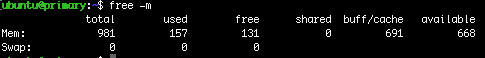
\includegraphics[width=0.8\linewidth]{images/worksheet_6_solution_1.png}
    \end{center}


    Using this information, I can write that the computer has

    \bigskip

    \begin{itemize}
        \item 981 MB of total memory
        \item 131 MB of free memory
    \end{itemize}

    \bigskip

    Second, I need to answer if these numbers match my intuition.

    \bigskip

    It does match my inution that free memory should be less than
    total memory.

    \bigskip

    \underline{\textbf{Notes}}

    \begin{itemize}
        \item I should ask professor the type of intution the author was expecting
        \item Installing Ubuntu Virtual Machine link: \href{https://multipass.run/}{here}
        \item Start virtual machine by typing command: \texttt{multipass start ubuntu-lts}
    \end{itemize}

    \item

    I need to write a little program \texttt{question\_3.c} (I will create this instead of
    \texttt{memory-user.c} for recording keeping purposes) that uses a certain amount of memory.

    \bigskip

    It's critera are:

    \begin{itemize}
        \item The program should take one command-line argument: the number of megabytes of memory it will use.
        \item The program should allocate an array.
        \item The program should constantly stream through the array, touching each entry.
        \item The program should do this indefinitely, or for a certain amount of time also specified in command line.
    \end{itemize}

    \bigskip

    For it's solution, please referr to \texttt{question\_3.c}

    \bigskip

    \underline{\textbf{Notes}}

    \begin{itemize}
        \item Learned that a large array ($> 5000$) can be generated using heap
        memory $^{[1]}$


        \item \textbf{Command Line Arguements in C}

        \begin{center}
        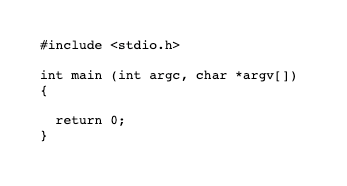
\includegraphics[width=0.7\linewidth]{images/worksheet_6_solution_2.png}
        \end{center}

        \begin{itemize}
            \item \texttt{argc}
            \begin{itemize}
                \item Is the number of arguments passed to the program
            \end{itemize}
            \item \texttt{argv}
            \begin{itemize}
                \item Is an array of strings
                \item Each string represents one of the arguements passed to the program
            \end{itemize}

            \bigskip

            \underline{\textbf{Example}}

            \bigskip

            \begin{center}
            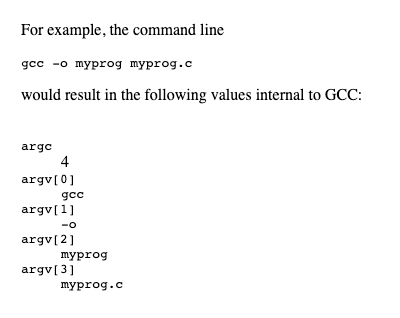
\includegraphics[width=0.7\linewidth]{images/worksheet_6_solution_3.png}
            \end{center}
        \end{itemize}

        \item \textbf{String to integer}

        \begin{itemize}
            \item \textbf{Syntax:} \texttt{int atoi(const char *string)}

            \bigskip

            \underline{\textbf{Example}}

            \bigskip

            \texttt{int output = atoi("20") /* Stores 20 in output*/}
        \end{itemize}
    \end{itemize}

    \bigskip

    \underline{\textbf{References}}

    \bigskip

    \begin{enumerate}[1)]
        \item Stackoverflow, Allocating A Large (5000+) Array, \href{https://stackoverflow.com/questions/5746377/allocating-a-large-5000-array}{link}
        \item Techdelight.com. Hpw tp fomd execution time of a C program, \href{https://www.techiedelight.com/find-execution-time-c-program/}{link}
        \item Stackoverflow, How do you clear the console screen in C, \href{https://stackoverflow.com/questions/2347770/how-do-you-clear-the-console-screen-in-c}{link}
    \end{enumerate}

    \item

    First, I need to revise program made in question 3 to also run the \texttt{free}
    tool.

    \bigskip

    For it's solution, please referr to \texttt{question\_4.c}.

    \bigskip

    Second, I need to answer how the memory is changing when the programming is running.

    \bigskip

    As program runs, the amount of memory available for the program decreases.

    \bigskip

    Once it runs out, it returns "Resource temporarily unavailable" error.

    \bigskip

    Third, I need to answer what happens to memory when program is killed.

    \bigskip

    In the current solution, I am using heap memory, and I haven't set it up
    for the array to be freed on kill signal. So, the lost memory is not reclaimed once killed.

    \bigskip

    Fourth, I need to answer what happens when a large amount of memory is used.

    \bigskip

    The answer is the same as second part of the question. It tries to fill up, but
    once available memory runs out, it force terminates with "Resource unavailable"
    error.


    \begin{center}
    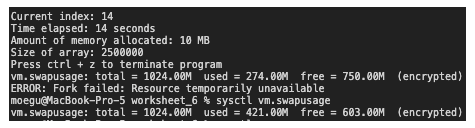
\includegraphics[width=\linewidth]{images/worksheet_6_solution_4.png}
    \end{center}

    \underline{\textbf{Notes}}

    \begin{itemize}
        \item Mac's equivalent of Ubuntu's \texttt{free -m} is \texttt{sysctl vm.swapusage} $^{[1]}$
    \end{itemize}

    \bigskip

    \underline{\textbf{References}}

    \begin{enumerate}[1)]
        \item Stack Overflow, Is there a Mac OS X Terminal version of the “free” command in Linux systems? ,\href{https://apple.stackexchange.com/questions/4286/is-there-a-mac-os-x-terminal-version-of-the-free-command-in-linux-systems/4296}{link}
    \end{enumerate}

    \item Please see link \href{https://man7.org/linux/man-pages/man1/pmap.1.html}{here}

    \item

    \adjustbox{valign=t}{
    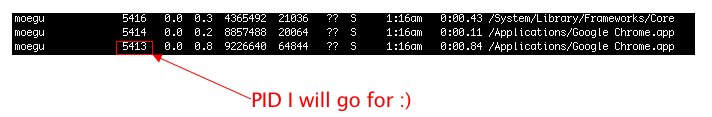
\includegraphics[width=\linewidth]{images/worksheet_6_solution_5.png}
    }

    \bigskip

    \underline{\textbf{Notes}}


    \begin{itemize}
        \item Alternative of pmap on Mac is \texttt{vmmap $<$PID$>$} $^{[1]}$
    \end{itemize}

    \bigskip

    \underline{\textbf{References}}

    \begin{enumerate}[1)]
        \item Yong Sun's Blog, Tips: the equivalents of ldd(1) and pmap(1) on Mac OS X, \href{http://yongsun.me/2009/01/tips-the-equivalents-of-ldd1-and-pmap1-on-mac-os-x/}{link}
    \end{enumerate}





\end{enumerate}

\end{document}